%! TEX root = 4_cantilever.tex
% the main TeX file which is intended to compile, :VimtexReload after adjustment
   % this file should be included in the main file
% :h vimtex-tex-root
\documentclass[../main.tex]{subfiles}
%ensure the class of docs

\begin{document}

\section{Struktur cantilever}%
\label{sec:section name}

Struktur cantilever slab atau plat cantilever adalah suatu sistem struktur dimana pemikulan sistem lantai dari pusat inti pusat bangunan tinggi (core) akan memungkinkan sebuah ruang dalam bangunan bebas dari kolom contohnya seperti aula ataupun sebuah show room, yang batas kekuatannya adalah batas terbesar ukuran bangunan dimana perhitungan dan pemilihan material yang digunakan adalah meterial yang kaku. Terutama apabila proyek si plat adalah besar kekuatan dapat ditingkatkan dengan menggunakan teknik pra-tekan.

\begin{figure}
	\begin{center}
		
\includegraphics[width=.82\textwidth]{detail_kantilever}
		% filename may not contain space but _
	\end{center}
	\caption{Detail Cantilever}
	\label{fig:detail_canti}
\end{figure}


Cantilever Slab Structure adalah hubungan struktur antara bidang penjepit dengan yang dijepit, terjadi pada salah satu pangkalnya saja, sehingga cenderung ujung yang lain menggantung sehingga memungkinkan ruang yang lebar dan bebas kolom.

Namun demikian struktur ini mempunyai keterbatasan, dalam hal beban yang ditimbulkan oleh bidang yang menggantung dan berhubungan dimensi bidang tersebut (tebal, panjang, lebar, dan lain-lain)

\subsection{Macam-Macam Bentuk Struktur Cantilever Slab}%
\label{sub:Macam-Macam Bentuk Struktur Cantilever Slab}

Yang dimaksud dengan struktur cantilever satu sisi dan struktur cantilever dua sisi adalah cantilever yang terdapat pada bangnan tinggi, yang berstruktur rangka. Jadi cantilever bukan sebagai struktur utama tapi hanya pada tepi bangunan dimana letak kolom lebih kedalam dari batas lantai 2 dinding.

\begin{figure}
	\begin{center}
		
\includegraphics[width=.82\textwidth]{macam_canti}
		% filename may not contain space but _
	\end{center}
	\caption{Macam-macam bentuk Struktur Cantilever}
	\label{fig:macam_canti}
\end{figure}

Secara umum dapat dijelaskan sebagai berikut tampak dari diagram datar bahwa kolom sudut itu hanya memikul antara 10-20\% dari beban vertikal yang dipikul oleh kolom-kolom tengah yang memikul posisi paling berat. Hal-hal diatas mendasari adanya cantilever satu sisi dan dua sisi Dari ilmu statistika, pemecahannya dengan melewatkan bagian bangunan diatas lantai atas sedemikian rupa sehingga kolom-kolom akhir mendapat pembebanan yang hampir sama dengan kolom-kolom ditengah. Semua kolom itu membuat kontras dengan satu sisi pendek bangunan yang nyatanya tanpa kolom-kolom sudut.


\tabitem Cantilever satu sisi

Pada gambar~\ref{fig:canti_satu_sisi} menunjukkan distribusi beban pada kerangka grid lebar yang lantai-lantainya diberi tonjolan konsol/kantilever disepanjang pendek bangunan, sedangkan kolom-kolom disepanjang bangunan tetap berada dalam permukaan bangunan.

Cantilever bersisi satu ini juga memperkaya komposisi arsitektural sebagai hasil untuk ciri yang diperlukan untuk membedakan berbagai tampak.
\begin{figure}
	\begin{center}
		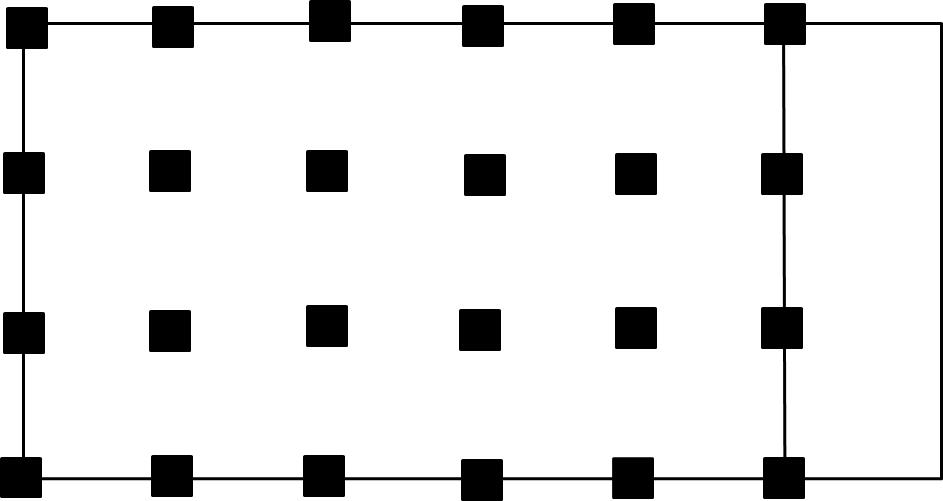
\includegraphics[width=.86\textwidth]{../figures/satu_sisi_canti.png}
		% filename may not contain space but _
	\end{center}
	\caption{Cantilever satu sisi}
	\label{fig:canti_satu_sisi}
\end{figure}


Cantilever satu sisi berhubungan erat dengan penyusunan kembali tampak pada sisi panjang dari sistem pendek bangunan. Hal-hal yang perlu diperhatikan sebagai berikut :

\begin{itemize}
	\item Sebuah balok cantilever yang bebas tidaklah dengan sendirinya bentuk struktur yang fasih
	\item Diperhitungkan bagaimana pembebanannya, dimana menonjolnya, bagaimana menahannya dan hubungan antara bentangan cantilever dan struktur pendukung.
	\item Balok cantilever harus dihubungkan secara organis kerangkanya, sebab balok cantilever dan rangka bangunan merupakan satu kesatuan yang rigid (kaku) dan monolit.
	\item Bila cantilever mempunyai proporsi yang sama, maka akan terjadi perkembangan yang wajar dari dimensi konstruksi lantai.
\end{itemize}

Gambar~\ref{fig:canti_satu_sisi} menunjukkan tampak kerangka dengan jarak kolom yang tepat dengan variasi cantilever serta penyesuaian dengan momen negatif. Momen cantilever ditempat dukung harus mempunyai hubungan yang amat tentu dengan momen lengkung pada balok bentang lain.

Apabila penonjolan cantilever amat kecil maka ekspresinya akan hilang, walaupun unsur strukturnya tidak terlihat. Tentunya pada keadaan tertentu cantilever yang amat kecil dengan murni meyakinkan logika fungsionalnya. Pada gambar dibawah ini penonjolan cantilever ditentukan oleh tebalnya tembok dinding yang padat hal ini mampu menahan gaya angin.

Cantilever sukar diterapkan dalam konstruksi grid sempit. Dalam struktur grid lebar cantilever dapat dinyatakan dengan kuat dan fasih.

\tabitem Cantilever dua sisi

Dalam struktur rangka kecuali cantilever di satu sisi dapat pula dipasang cantilever dikedua sisi sudut bangunan bagian atas. Gambar disamping menunjukkan bagaimana cara rangka grid lebar membagi ratakan beban pada kolom-kolom berikut yakni kolom sudut. Disini kolom sudut mendapat bagian beban yang sama dideretan kolom tengah.

Pemberian cantilever ini pada grid sempit tidaklah cocok, karena jarak kolom ke arah memanjang terlalu dekat untuk memenuhi keperluan didalam. Pada gambar dilihat beberapa bangunan dengan cantilever dikedua sisi. Disini kerangka diundurkan dari semua tampak dan hanya dapat dibedakan dari luar, karena bidang-bidang jendela dibuat transparan.

Ekspresi tampak berasal dari dinding tirai yang geometris yang dalam perencanaan seorang arsitek mempunyai kebebasan yang sempurna. Dalam gambar disamping tampak ringan hanya seolah-olah digantung secara serampangan pada kerangka. Dalam hal ini tergantung dari pemeliharaan, hubungan yang baik antara kulit luar dan rangka pendukung.

Apabila dinding tirai dibuat dari rangka padat, maka akan terkesan berat dan tidak adanya kesatuan antara bagian luar dan kerangka yang didalam. Cantilever dua sisi memberikan kesempatan yag sama dalam pemecahan masalah seperti juga pada cantilever satu sisi.

\begin{figure}
	\begin{center}
		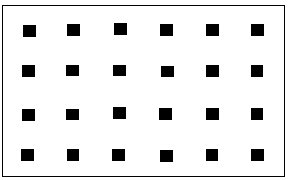
\includegraphics[width=.82\textwidth]{../figures/dua_sisi.png}
		% filename may not contain space but _
	\end{center}
	\caption{Struktur Cantilever Dua Sisi}
	\label{fig:dua_sisi}
\end{figure}

\subsection{Parameter dan Pertimbangan Struktur}%
\label{sub:Parameter dan Pertimbangan Struktur}

\subsubsection{Parameter Struktur}%
\label{ssub:Parameter Struktur}

\textbf{Kekuatan}

Sebuah bangunan haruslah mempunyai kekuatan untuk dapat berdiri. Kekuatan tegaknya suatu bangunan sangatlah tergantung pada jenis struktur yang digunakan, sehingga beban yang mungkin diterima oleh bangunan dapat diperkirakan dengan cara perhitungan matematis struktur. Hal ini perlu dilakukan guna menghindari terjadinya sebuah kecelakaan yang menyebabkan keugian baik materi maupun jiwa.

Selain itu dengan memperhitungkan sistem struktur terutama bangunan yang menggunakan struktur cantilever, maka bangunan tersebut sekiranya dapat menahan beban yang diterima. Pada perencanaan sebuah bangunan dikenal adanya beberapa jenis beban yang sekiranya dapat mempengaruhi bentuk, kekuatan, kestabilan dan keseimbangan dari bangunan tersebut. Penanganan terhadap faktor diatas dapat dijelaskan sebagai berikut :

\begin{itemize}
	\item Pada kolom yang tertinggi dengan beban sentris pada sumbu balok mengakibatkan batang kolom mengalami tekuk akibat gaya yang bekerja. Besarnya tekuk yang terjadi sangat bergantung pada besarnya beban yang bekerja serta material yang digunakan.
	\item Hal ini berlaku juga untuk struktur utama pada sebuah bangunan. Misalnya sebuah bangunan menggunakan Cantilever Slab sebagai struktur utama, maka elemen struktur bergerak sehingga menyebabkan terjadinya dari reaksi partikel-partikel struktur cantilever.
	\item Karena dimensi yang tidak tepat dari struktur cantilever maka elemen struktur bergerak mengikuti arah beban luar yang bergerak (terjadi tekuk).
\end{itemize}

Agar elemen struktur mampu memikul beban yang terjadi, maka dimensi yang melawan gaya tarik akibat gaya luar diperbesar sehingga elemen struktur dapat menahan beban yang terjadi.

Struktur cantilever slap adalah hubungan struktur antara bidang penjepit dengan bagian yang dijepit dan terjadi pada bagian pangkalnya, sehigga ujung yang lain tergantung. Pemikul sistem lantai dari sebuah bangunan dengan sistem cantilever akan memungkinkan adanya ruang yang bebas terhadap kolom dengan kekuatannya sama besar dengan besarnya ukuran ruang yang dimaksud. Kekakuan plat dapat ditingkatkan dengan menggunakan teknik-teknik struktur pra-tekan

Struktur rangka tinggi pada lantai yang tercantilever pada setiap lantai memungkinkan adanya ruang yang fleksibel didalam dan diatas rangka. Sistem gantung memungkinkan memungkinkan penggunaan bahan secara efisien dengan menggunakan penggantung sebagai pengganti kolom, untuk memikul beban lantai.

Kekuatan unsur tekan harus dikurangi karena adanya bahaya tekuk. Berbeda dengan unsur tarik yang dapat mendayagunakan kemampuannya secara maksimal, kabel-kabel penggantung meneruskan ke rangka dibagian atas yang tercantilever dari inti pusat:

\begin{figure}
	\begin{center}
		
\includegraphics[width=.82\textwidth]{cth_canti}
		% filename may not contain space but _
	\end{center}
	\caption{Contoh Struktur Terkantilever}
	\label{fig:cth_canti}
\end{figure}


\textbf{Kestabilan}

Kestabilan dapat tercapai apabila bentuk bangunan secara keseluruhan mampu menahan gaya yang berasal dari luar (gaya lateral) yang disebabkan oleh gaya angin dan gempa. Untuk mengatasi gaya tersebut diatas digunakan penyelesaian sistem struktur pada struktur lantai.

\begin{figure}
	\begin{center}
		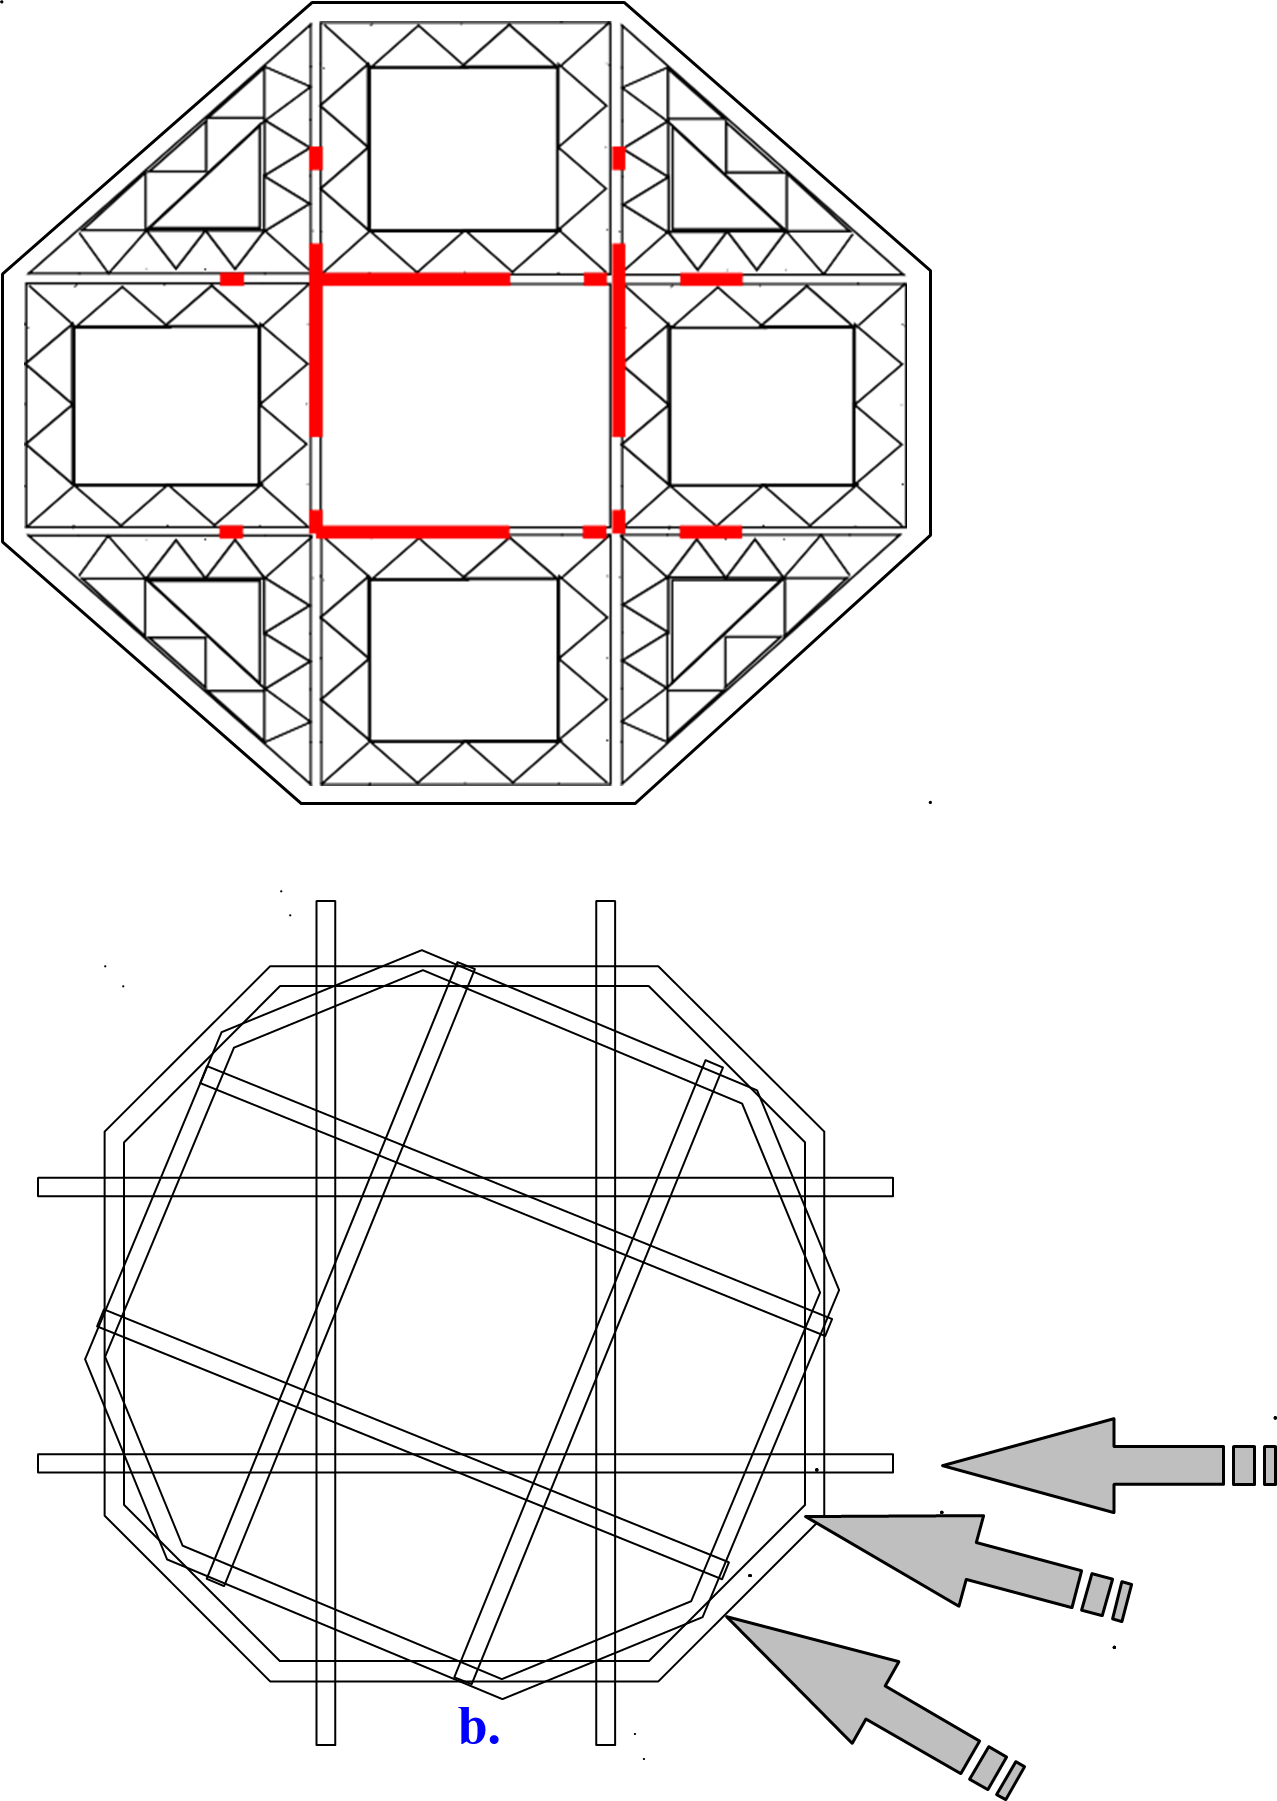
\includegraphics[width=.82\textwidth]{../figures/stabil_canti.png}
		% filename may not contain space but _
	\end{center}
	\caption{Susunan Balok dalam menjaga Kestabilan bangunan}
	\label{fig:stabil_canti}
\end{figure}

Untuk meniadakan puntiran akibat angin, maka pada struktur lantai dipasang balok pengikat (brancing), brancing horisontal dipilih untuk menahan gaya lateral yang mengenai bidang bangunan. Dimana bracing ini berfungsi sebagai pengaku struktur pada bangunan.

Gaya-gaya pada bracing dalam arah diagonal akan melawan gaya lateral, sehingga resultan gaya menjadi seimbang atau sama dengan 0 (nol).

Dengan demikian balok pengikat cukup diletakkan di tepi-tepi bidang lantai. Karena bidang tepi berhubungan dengan gaya luar (gaya lateral).

\begin{itemize}
	\item Bila gaya lateral yang mengenai bangunan dengan arah yang sejajar, maka akan menimbulkan flutering atau puntiran pada bangunan.
	\item Sedangkan untuk mengakukan letak kolom struktur akibat gaya lateral yang terjadi, digunakan balok pengikat yang dihubungkan dengan balok-balok utama, sehingga gaya lateral dapat ditiadakan oleh balok pengikat. Dengan menggunakan cara ini maka bangunan akan dapat menahan beban yang ditimbulkan oleh gaya lateral.
\end{itemize}

\textbf{Keseimbangan}

Upaya menciptakan suatu bentuk yang mampu berdiri sendiri, yang disebabkan oleh gaya gravitasi. Untuk dapat mencapai kondisi yang seimbang, dalam menyelesaikan sistem struktur sebuah bangunan adalah :

\begin{itemize}
	\item Balok sebagai struktur pendukung dengan perletakan bebas pada ujungnnya dan terjepit pada ujung yang lain, akan membentuk momen terbesar pada ujung yang bebas. Maka bentuk sistem struktur yang paling tepat untuk bangunan seperti ini adalah sistem struktur cantilever.
	\item Akibat memerlukan ruang cukup luas, maka sistem cantilever dengan bentangan yang cukup luas, panjang dan dimana pada salah satu ujungnya bebas dimungkinkan terjadinya tekuk akibat beban yang diterima atau dipikul maka perlu adanya penanganan khusus yaitu dengan cara menggunakan kabel baja sebagai pengaku yang dipasang pada ujung bebas dari struktur cantilever dengan tiang kolom sebagai pendukung utama atau pengaku bangunan.
	\item Penggunaan material yang tipis akan melekuk pada arah gaya tekan diikuti oleh elemen lain yang berhubungan dengannya. Oleh karena itu timbul puntiran dengan menggabungkan kedua elemen struktur cantilever dengan balok tarik pada ujung kolom dan balok tekan pada bagian tengah kolom sebagai perlawanan dari pergerakan elemen struktur cantilever.
	\item Dengan penggabungan dua elemen struktur cantilever melalui balok penghunbung (tarik-tekan) diperoleh satu bentuk struktur yang seimbang.
\end{itemize}

\begin{figure}
	\begin{center}
		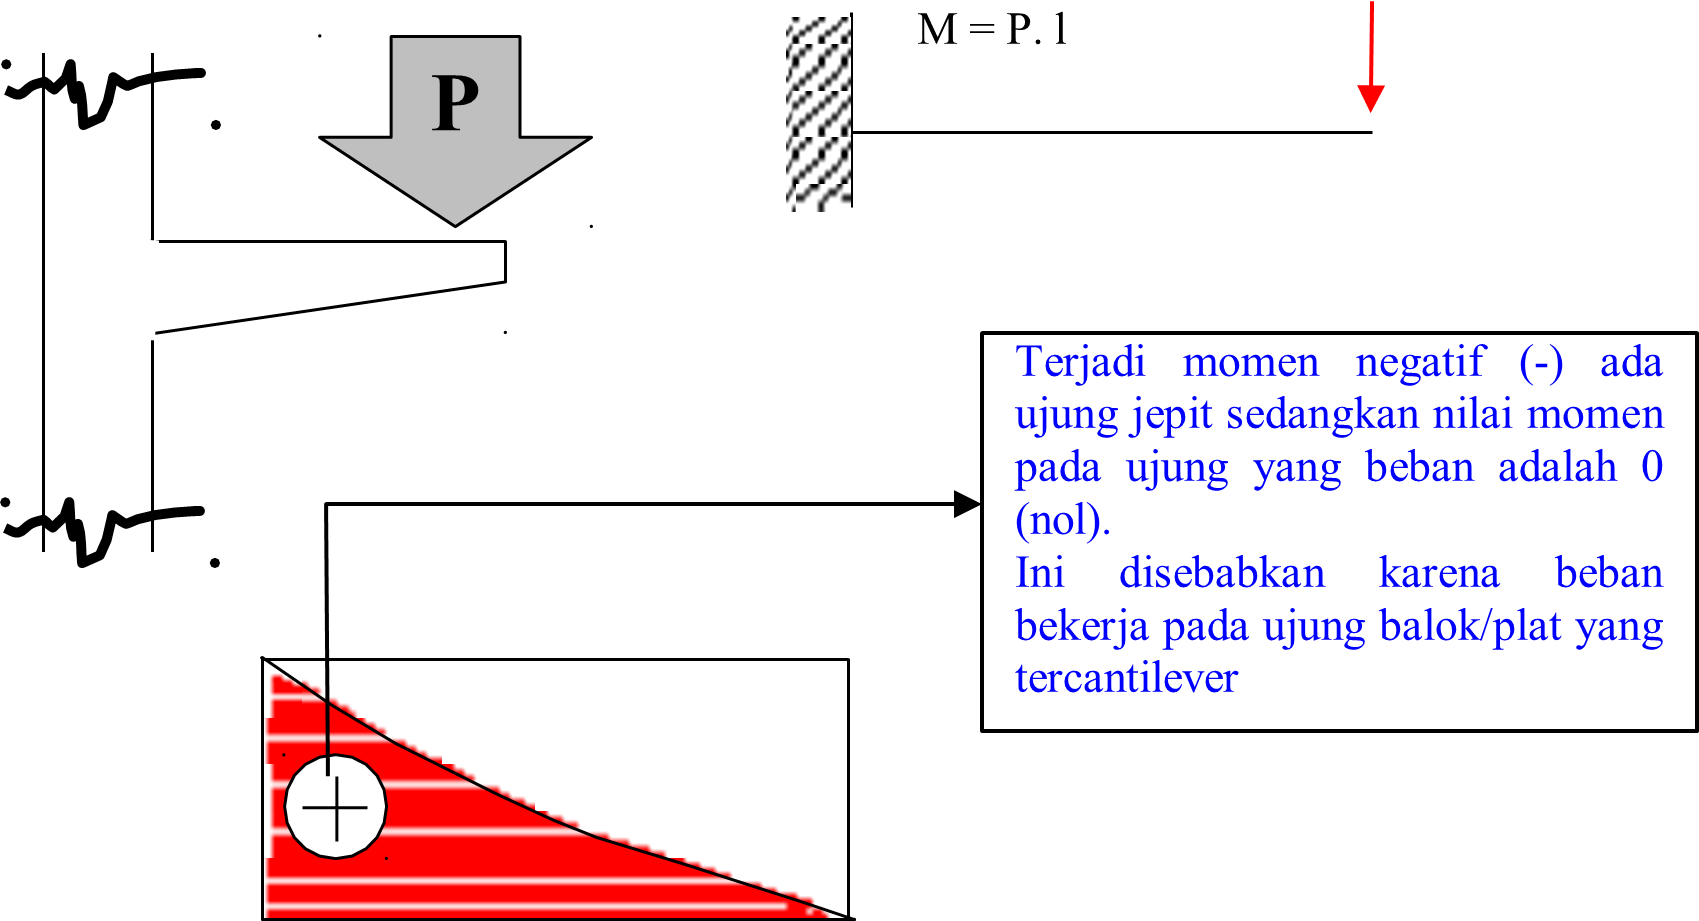
\includegraphics[width=.82\textwidth]{../figures/seimbang_canti.png}
		% filename may not contain space but _
	\end{center}
	\caption{Bentuk Analisis Keseimbangan Cantilever}
	\label{fig:seimbang_canti}
\end{figure}

\begin{figure}
	\begin{center}
		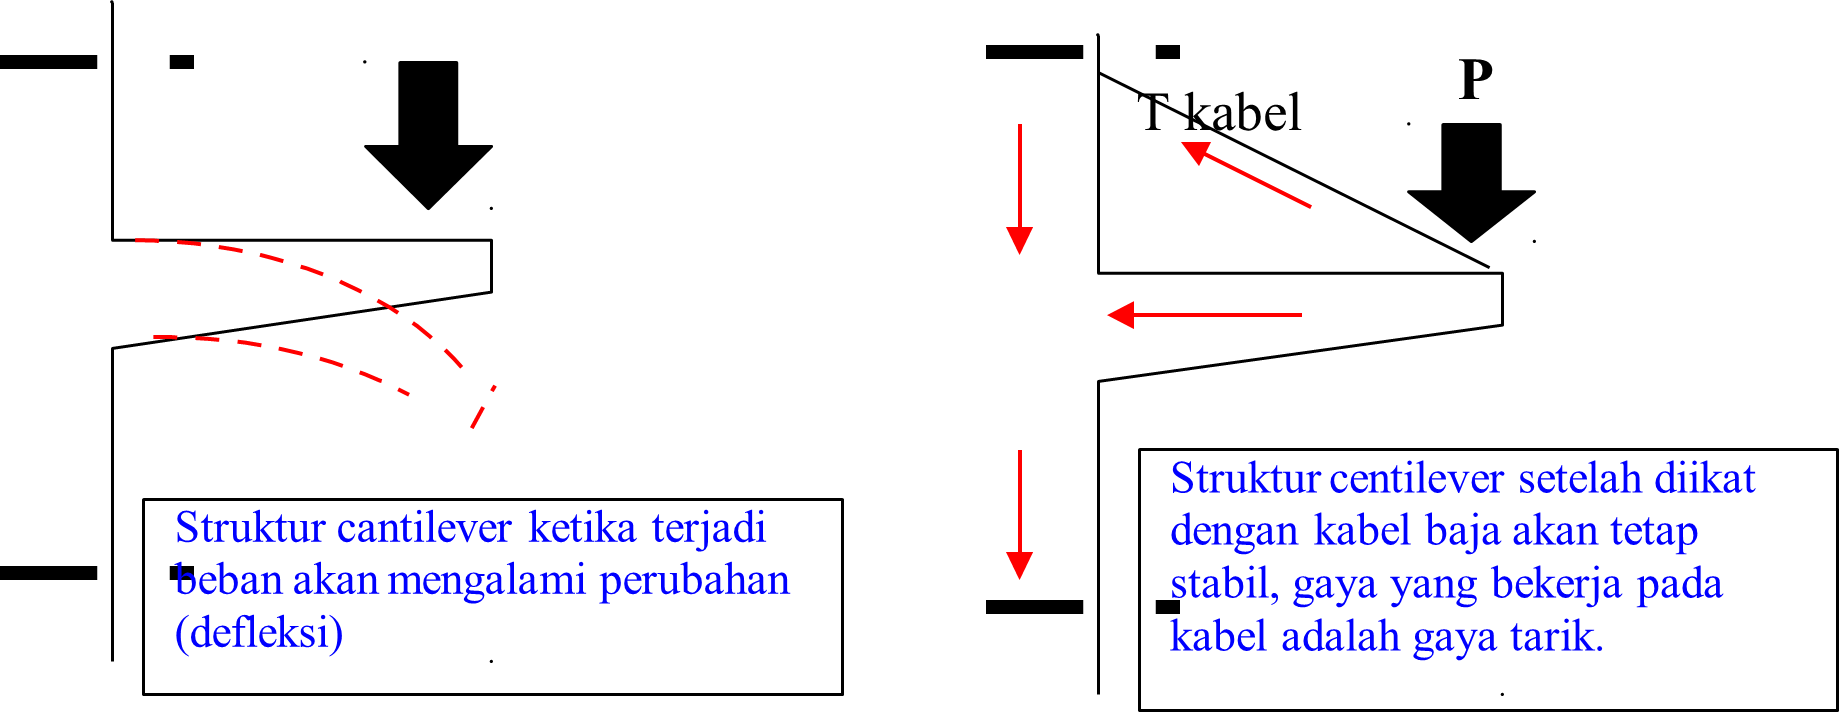
\includegraphics[width=.82\textwidth]{../figures/defleksi_canti.png}
		% filename may not contain space but _
	\end{center}
	\caption{Defkelsi Struktur Cantilever}
	\label{fig:defleksi_canti}
\end{figure}

\begin{figure}
	\begin{center}
		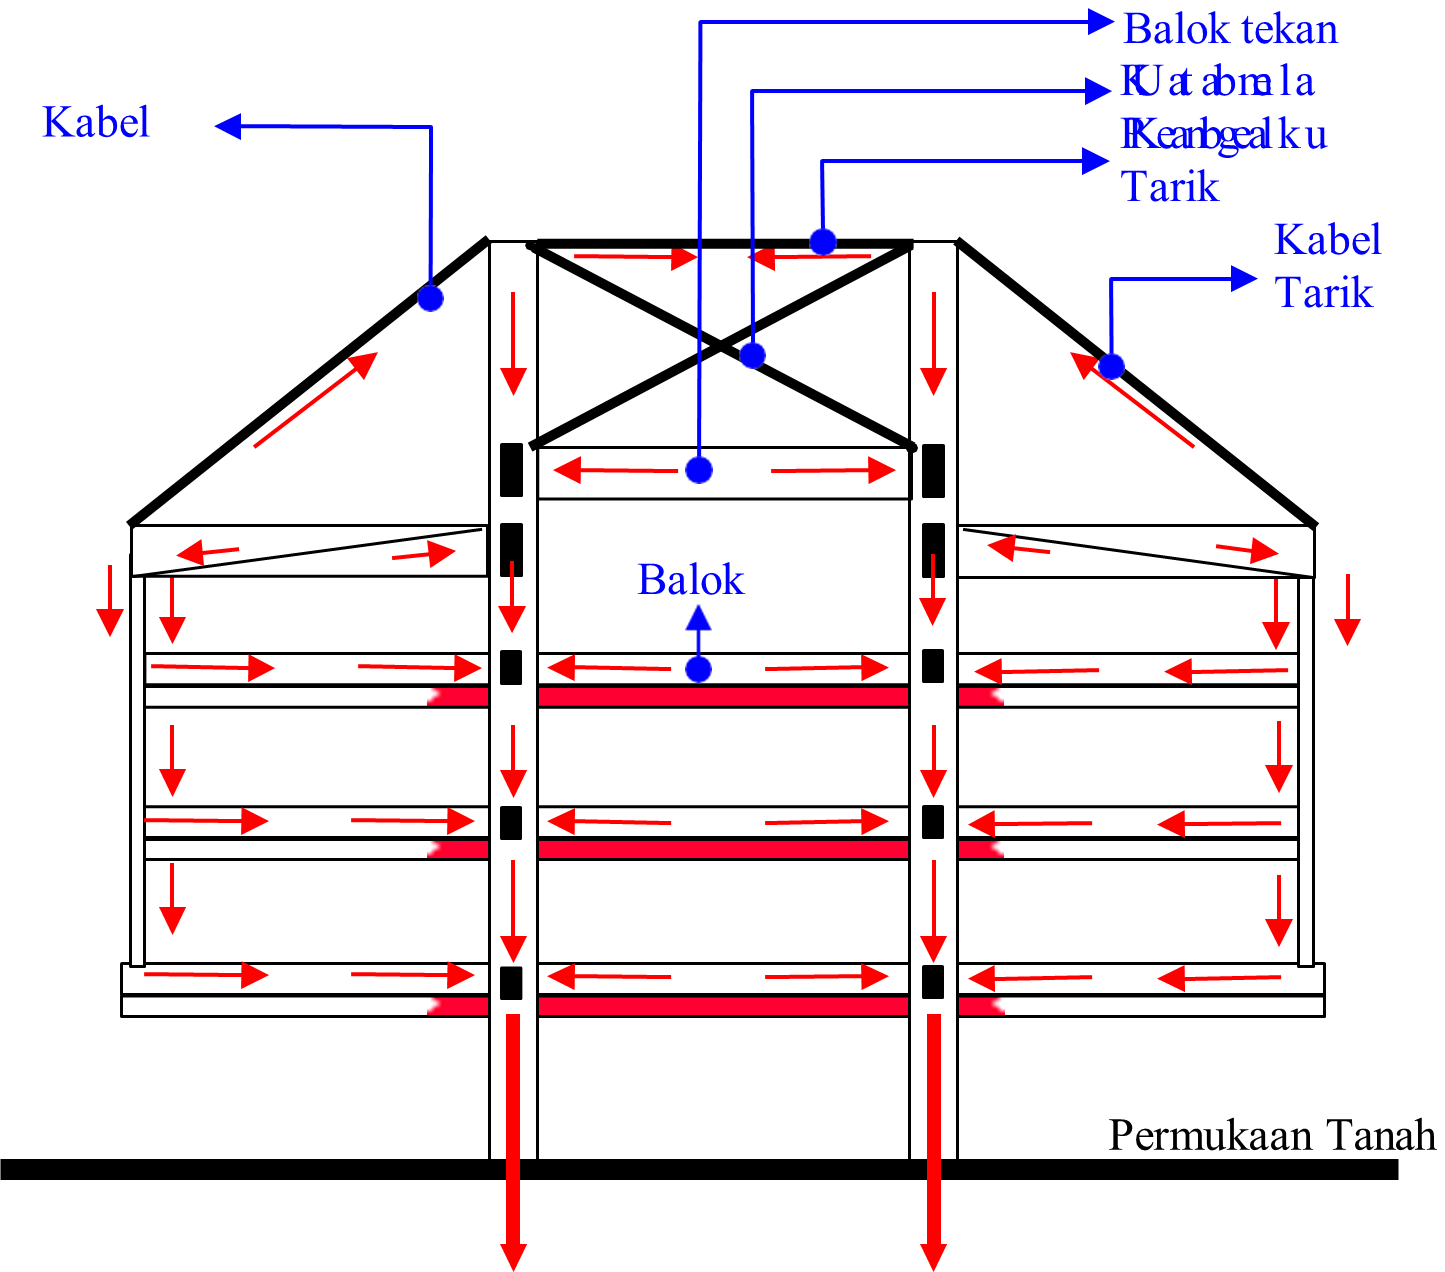
\includegraphics[width=.82\textwidth]{../figures/penyaluran_gaya.png}
		% filename may not contain space but _
	\end{center}
	\caption{Struktur Cantilever Gabungan 2 Elemen dan pola penyaluran gaya}
	\label{fig:salur_gaya}
\end{figure}


\subsubsection{Pertimbangan Struktur}%
\label{ssub:Pertimbangan Struktur}
\begin{itemize}
	\item Ekonomi
	\item Kondisi Tanah
	\item Pabrikasi dan Pembangunan
	\item Pertimbangan Mekanis
	\item Pertimbangan Rasio Tinggi-Lebar Suatu Bangunan
	\item Pertimbangan Tingkat Bahaya Kebakaran
	\item Pertimbangan Lingkungan/Setempat
\end{itemize}



























\bibliographystyle{apalike}
\bibliography{../filename.bib} % required for citecompletion, not work in mainfile
\end{document}

